%%%%%%%%%%%%%%%%%%%%%%%%%%%%%%%%%%%%%%%%%%%%%%%%%%%%%%%%%%%%%%%%%%%%%%%%%%%%%%%
%                         CAPITULO 7
%                  Proyecto Academico
%%%%%%%%%%%%%%%%%%%%%%%%%%%%%%%%%%%%%%%%%%%%%%%%%%%%%%%%%%%%%%%%%%%%%%%%%%%%%%%

%=============================================================================
% MARCA VISUAL DE SEPARACION: este capitulo describe el proyecto practico
% de la asignatura, con tematica y enfoque diferenciados.
%=============================================================================

{\centering\noindent\rule{\textwidth}{1pt}\par}

\begin{center}
\Large\textbf{PROYECTO ACADEMICO}
\end{center}

{\centering\noindent\rule{\textwidth}{1pt}\par}

\vspace{0.5cm}

\begin{center}
\fbox{\parbox{0.9\textwidth}{\centering\emph{A partir de este punto se describe el proyecto practico de la asignatura: un sistema de automatizacion distribuido con ESP32, Arduino UNO y comunicacion MQTT. El contenido y la estructura de este capitulo difieren de los anteriores, reflejando el caracter aplicado del trabajo.}}}
\end{center}

\vspace{0.5cm}

\chapter{Proyecto Academico: Automatizacion con ESP32, Arduino UNO y MQTT}

El presente capitulo recoge la memoria tecnica del proyecto de automatizacion desarrollado en el marco de la asignatura. El sistema consiste en una arquitectura distribuida de tres microcontroladores interconectados mediante bus I2C, con un ESP32 Master que actua como gateway WiFi/MQTT hacia un broker externo, y una plataforma de visualizacion y persistencia basada en Node-RED y MongoDB.

A lo largo del capitulo se describen los subsistemas de hardware y firmware, los protocolos de comunicacion empleados (I2C y MQTT), la maquina de estados que gobierna la logica de control, las versiones de simulacion desarrolladas para validacion sin hardware, y los problemas detectados y corregidos durante el desarrollo.


\section{Resumen Ejecutivo}

El proyecto consiste en un sistema de automatizacion distribuido compuesto por tres microcontroladores interconectados mediante bus I2C y un ESP32 Master que actua como gateway WiFi/MQTT hacia un broker externo. El sistema gestiona sensores de presencia y nivel de agua, y controla actuadores (motores y bomba) segun una maquina de estados centralizada. Se han implementado versiones de produccion y versiones de simulacion para validacion sin hardware de sensores.

\begin{definicion}
El sistema sigue una \textbf{arquitectura de tres capas}: capa de adquisicion (firmware embebido en ESP32 y Arduino UNO), capa de transporte (MQTT sobre TCP/IP) y capa de orquestacion, visualizacion y persistencia (Node-RED + MongoDB).
\end{definicion}


\section{Objetivo del Proyecto}

El objetivo funcional del sistema es automatizar un proceso industrial o agricola con las siguientes caracteristicas:

\begin{itemize}
    \item \textbf{Deteccion de presencia}: mediante un sensor conectado al ESP32 Slave.
    \item \textbf{Medicion de nivel de agua}: mediante un sensor analogico conectado al Arduino UNO Slave.
    \item \textbf{Control de motores}: cuatro motores controlados por el ESP32 Slave.
    \item \textbf{Control de bomba de agua}: una bomba controlada por el Arduino UNO Slave.
    \item \textbf{Supervision remota}: publicacion del estado del sistema via MQTT para monitorizacion externa.
    \item \textbf{Logica centralizada}: el Master ESP32 toma todas las decisiones; los esclavos actuan como unidades de entrada/salida remotas.
\end{itemize}


\section{Arquitectura General del Sistema}

El sistema simula una linea de produccion compuesta por tres etapas principales:
\begin{itemize}
    \item Control de nivel de tanque
    \item Sistema de llenado
    \item Transporte de botellas
\end{itemize}
Cada etapa esta controlada por nodos (ESP32 Wroover / Arduino UNO), que se comunican mediante protocolo I2C.

\begin{figure}[H]
\centering
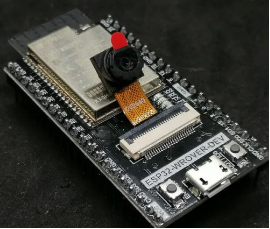
\includegraphics[width=0.6\textwidth]{assets/cap7/7.1.png}
\caption{ESP32 Wroover}
\label{fig:esp32-img}
\end{figure}

\begin{figure}[H]
\centering
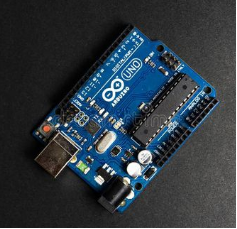
\includegraphics[width=0.6\textwidth]{assets/cap7/7.2.png}
\caption{Arduino UNO}
\label{fig:arduino-img}
\end{figure}

\begin{figure}[H]
\centering
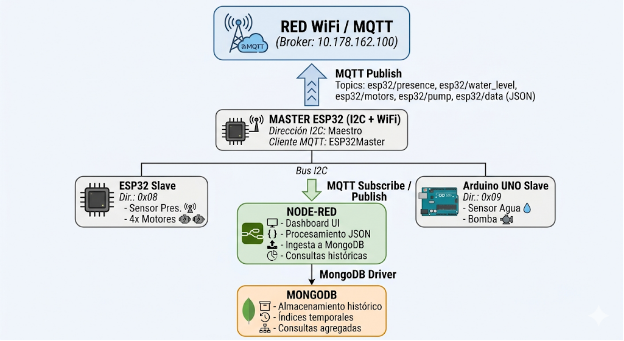
\includegraphics[width=0.95\textwidth]{assets/cap7/7.3.png}
\caption{Esquema de funcionamiento del sistema}
\label{fig:esquema-funcionamiento}
\end{figure}

\textbf{Comunicacion I2C:} Un Maestro (Master ESP32) y dos Esclavos (ESP32 Slave y Arduino UNO Slave) se comunican mediante los pines SCL y SDA. El bus es half-duplex.

\textbf{Topologia MQTT:} El Master ESP32 es el unico productor (publisher). Node-RED actua como suscriptor/consumer principal y se encarga de anadir y consultar la base de datos MongoDB.

\textbf{Flujo de datos principal:}

\begin{figure}[H]
\centering
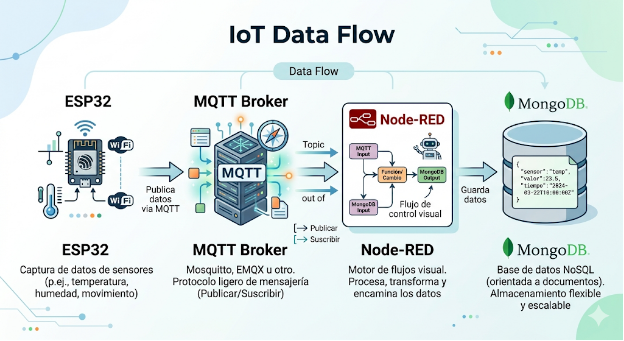
\includegraphics[width=0.95\textwidth]{assets/cap7/7.4.png}
\caption{Flujo de datos principal del sistema}
\label{fig:flujo-datos}
\end{figure}





\section{Protocolo de Comunicacion I2C}

\subsection{Parametros del Bus}

\begin{table}[H]
\centering
\small
\caption{Parametros del bus I2C}
\label{tab:i2c-parametros}
\begin{tabularx}{0.6\textwidth}{@{}lX@{}}
\toprule
\textbf{Parametro} & \textbf{Valor} \\
\midrule
Modo & Maestro-Esclavo \\
Frecuencia & 100 kHz (Standard Mode) \\
Pull-ups & Externas (en hardware) \\
\bottomrule
\end{tabularx}
\end{table}

\subsection{Transacciones}

Transacciones iniciadas por el Master en cada ciclo de \texttt{loop()} (periodo aproximado 200 ms):

\begin{table}[H]
\centering
\small
\caption{Transacciones I2C del ciclo principal}
\label{tab:i2c-transacciones}
\begin{tabularx}{0.85\textwidth}{@{}cclX@{}}
\toprule
\textbf{Orden} & \textbf{Dir.} & \textbf{Bytes} & \textbf{Descripcion} \\
\midrule
1 & 0x08 & 1 & Lectura presencia \\
2 & 0x09 & 2 & Lectura nivel agua + estado bomba \\
3 & 0x08 & 1 & Escritura comando motor (\texttt{'E'} / \texttt{'D'}) \\
4 & 0x09 & 1 & Escritura comando bomba (\texttt{'O'} / \texttt{'F'}) \\
\bottomrule
\end{tabularx}
\end{table}

Las escrituras (pasos 3 y 4) solo se ejecutan si el estado objetivo difiere del ultimo envio exitoso (optimizacion anti-spam).

\subsection{Protocolo de Aplicacion (Comandos)}

\begin{table}[H]
\centering
\small
\caption{Comandos del protocolo de aplicacion I2C}
\label{tab:i2c-comandos}
\begin{tabularx}{\textwidth}{@{}lccc@{}}
\toprule
\textbf{Esclavo} & \textbf{Comando} & \textbf{Valor} & \textbf{Accion} \\
\midrule
ESP32 (0x08) & \texttt{'E'} & Enable & Encender los 4 motores \\
ESP32 (0x08) & \texttt{'D'} & Disable & Apagar los 4 motores \\
Arduino (0x09) & \texttt{'O'} & ON & Encender bomba \\
Arduino (0x09) & \texttt{'F'} & OFF & Apagar bomba \\
\bottomrule
\end{tabularx}
\end{table}

\subsection{Manejo de Errores I2C}

Implementado en el Master:
\begin{itemize}
    \item \textbf{Lecturas:} Hasta 3 reintentos si \texttt{requestFrom} no devuelve la cantidad de bytes esperada.
    \item \textbf{Escrituras:} Hasta 2 reintentos si \texttt{endTransmission} devuelve error (diferente de 0).
    \item Delay entre reintentos: 500 µs (\texttt{delayMicroseconds(500)}).
\end{itemize}


\section{Protocolo de Comunicacion MQTT}

\subsection{Broker y Conectividad}

\begin{table}[H]
\centering
\small
\caption{Configuracion del broker MQTT}
\label{tab:mqtt-broker}
\begin{tabularx}{0.7\textwidth}{@{}lX@{}}
\toprule
\textbf{Parametro} & \textbf{Valor} \\
\midrule
Broker IP & \texttt{10.178.162.100} (produccion/simulacion) \\
Puerto & 1883 \\
Client ID Master & \texttt{ESP32Master} / \texttt{ESP32MasterSim} \\
Keepalive & 60 s \\
\bottomrule
\end{tabularx}
\end{table}

\subsection{Topics Publicados}

\begin{table}[H]
\centering
\small
\caption{Topics MQTT publicados por el Master}
\label{tab:mqtt-topics}
\begin{tabularx}{\textwidth}{@{}lXX@{}}
\toprule
\textbf{Topic} & \textbf{Tipo de Payload} & \textbf{Descripcion} \\
\midrule
\texttt{esp32/presence} & \texttt{"1"} / \texttt{"0"} & Estado de presencia detectada \\
\texttt{esp32/water\_level} & \texttt{"0"} -- \texttt{"100"} & Nivel de agua mapeado \\
\texttt{esp32/motors} & \texttt{"1"} / \texttt{"0"} & Estado de los motores \\
\texttt{esp32/pump} & \texttt{"1"} / \texttt{"0"} & Estado de la bomba \\
\texttt{esp32/data} & JSON consolidado & Mensaje con todos los datos + timestamp + device\_id \\
\bottomrule
\end{tabularx}
\end{table}

\subsection{Formato del JSON Consolidado}

El topic \texttt{esp32/data} transporta un mensaje JSON con la siguiente estructura:

\begin{lstlisting}[caption={Formato del JSON consolidado en esp32/data},label={lst:json-consolidado}]
{
  "device_id": "ESP32-Master",
  "timestamp": "2026-05-26T14:23:04Z",
  "presence": "DETECTED",
  "water_level": 95,
  "motors": "ON",
  "pump": "OFF"
}
\end{lstlisting}

El campo \texttt{timestamp} se envia como string ISO 8601 UTC. Para su correcta ingestion en MongoDB, el receptor (Node-RED) debe convertir la cadena a objeto \texttt{Date} antes de la insercion:

\begin{lstlisting}[caption={Conversion de timestamp en Node-RED},label={lst:conversion-timestamp}]
if (msg.payload && msg.payload.timestamp) {
    msg.payload.timestamp = new Date(msg.payload.timestamp);
}
return msg;
\end{lstlisting}


\section{Maquina de Estados del Sistema}

La logica de control reside integramente en el Master ESP32. Existen 4 estados:

\begin{table}[H]
\centering
\small
\caption{Maquina de estados del sistema}
\label{tab:maquina-estados}
\begin{tabularx}{\textwidth}{@{}lXXX@{}}
\toprule
\textbf{Estado} & \textbf{Descripcion} & \textbf{Motores} & \textbf{Bomba} \\
\midrule
\texttt{STATE\_RUNNING} & Operacion normal & ON & OFF \\
\texttt{STATE\_PUMP\_DELAY} & Espera antes de bombear & OFF & OFF \\
\texttt{STATE\_PUMPING} & Bomba activa & OFF & ON \\
\texttt{STATE\_RECOVERY} & Recuperacion antes de reiniciar & OFF & OFF \\
\bottomrule
\end{tabularx}
\end{table}
Durante \texttt{STATE\_PUMP\_DELAY}, si \texttt{waterLevel >= 35}, se activa la bomba y se pasa a \texttt{STATE\_PUMPING}. Si el nivel es inferior, se salta directamente a \texttt{STATE\_RECOVERY}.








\section{Arquitectura Software y Flujo de Datos}

El sistema implementa una arquitectura software distribuida en tres capas principales:

\begin{enumerate}
    \item \textbf{Capa de Adquisicion}: firmware embebido en los microcontroladores ESP32 y Arduino UNO. El Master ESP32 recopila datos de sensores y estados de actuadores mediante I2C.
    \item \textbf{Capa de Transporte}: el broker MQTT actua como bus de mensajes desacoplado, permitiendo monitorizacion en tiempo real e ingesta de datos historicos.
    \item \textbf{Capa de Orquestacion y Visualizacion}: Node-RED procesa los payloads JSON, distribuye la informacion al dashboard y gestiona la persistencia en MongoDB.
    \item \textbf{Capa de Persistencia}: MongoDB almacena los datos historicos para analisis temporal, generacion de informes y consultas.
\end{enumerate}

\textbf{Flujo de datos principal:} ESP32 (adquisicion) $\rightarrow$ MQTT (transporte) $\rightarrow$ Node-RED (procesamiento/visualizacion) $\rightarrow$ MongoDB (historizacion).


\section{Interfaz, Visualizacion y Dashboard}

El sistema utiliza \textbf{Node-RED Dashboard} como plataforma principal de visualizacion y supervision. Las interfaces graficas permiten visualizar las siguientes variables:

\begin{itemize}
    \item Nivel de agua del tanque (\texttt{water\_level})
    \item Estado de los motores (\texttt{motors})
    \item Estado de la bomba de agua (\texttt{pump})
    \item Deteccion de presencia (\texttt{presence})
    \item Variables recibidas desde los dispositivos ESP32 (identificador, timestamp, etc.)
\end{itemize}

\begin{figure}[H]
\centering
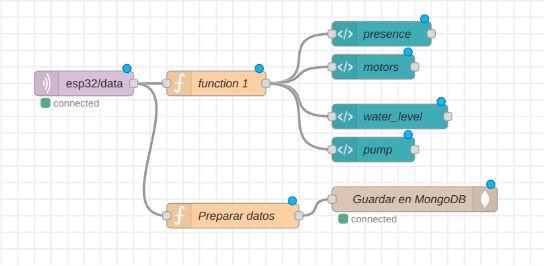
\includegraphics[width=0.8\textwidth]{assets/cap7/7.5.png}
\caption{Dashboard de Node-RED con visualizacion de variables del sistema}
\label{fig:dashboard-nodered}
\end{figure}

\subsection{Flujo de Adquisicion en Tiempo Real}

Flujo principal en Node-RED para suscripcion, procesamiento y visualizacion de datos:

\begin{enumerate}
    \item \textbf{Suscripcion MQTT:} se suscribe al topic \texttt{esp32/data}.
    \item \textbf{Recepcion JSON:} recibe el payload JSON consolidado.
    \item \textbf{Descomposicion:} extrae y procesa cada variable individualmente.
    \item \textbf{Visualizacion:} muestra cada dato mediante elementos visuales del dashboard.
\end{enumerate}

\begin{figure}[H]
\centering
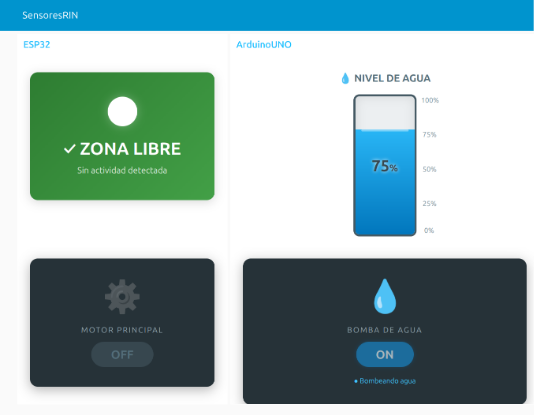
\includegraphics[width=0.8\textwidth]{assets/cap7/7.6.png}
\caption{Flujo de Node-RED para adquisicion en tiempo real}
\label{fig:flujo-nodered-tiempo-real}
\end{figure}

\subsection{Flujo de Analisis Historico}

\begin{figure}[H]
\centering
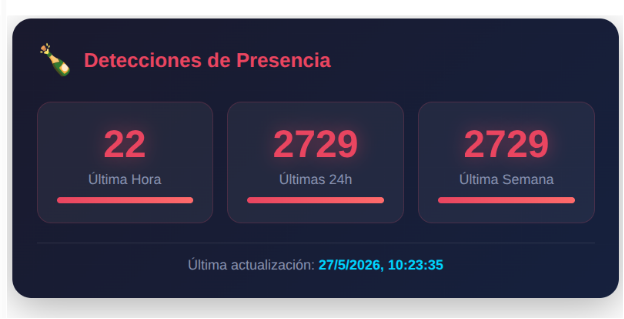
\includegraphics[width=0.8\textwidth]{assets/cap7/7.7.png}
\caption{Dashboard con contador de botellas}
\label{fig:dashboard-botellas}
\end{figure}

Flujo independiente dedicado a la lectura de datos desde MongoDB y presentacion de informacion historica en el dashboard. Proporciona:

\begin{itemize}
    \item Conteo de botellas detectadas (ultima hora, ultimo dia, ultima semana).
    \item Visualizacion simultanea de estadisticas en diferentes ventanas temporales.
    \item Consulta del timestamp de la ultima botella detectada.
\end{itemize}








\section{Diseno de Red Corporativa para la Planta Industrial}

Como parte del proyecto, se ha disenado e implementado en Cisco Packet Tracer un modelo de red corporativa que refleja la infraestructura de comunicaciones que daria soporte a la planta industrial descrita en este capitulo. El objetivo es simular la separacion entre los entornos OT (Operational Technology) e IT (Information Technology) y verificar la conectividad entre todos los elementos del sistema.

\subsection{Arquitectura de red}

La red se estructura en seis subredes, cada una con un proposito especifico:

\begin{itemize}
    \item \textbf{Red de produccion (OT)}: 192.168.10.0/24 — contiene los tres PLCs que controlan las etapas del proceso (control de tanque, llenado y transporte de botellas). Es la unica red con acceso directo a los dispositivos de campo.
    \item \textbf{Red de ingenieria}: 192.168.20.0/24 — estaciones de trabajo para el personal de mantenimiento y supervision tecnica de la linea.
    \item \textbf{Red de administracion}: 192.168.30.0/24 — puestos de gestion y ofimatica de la planta.
    \item \textbf{Red de servidores (DMZ)}: 192.168.40.0/24 — aloja los servidores MQTT Broker, Node-RED y MongoDB, actuando como zona desmilitarizada entre OT e IT.
    \item \textbf{Red de control de calidad}: 192.168.50.0/24 — puesto de inspeccion con camara IP para supervision visual.
    \item \textbf{Red WiFi corporativa}: 192.168.100.0/24 — acceso inalambrico para dispositivos moviles del personal.
\end{itemize}

\begin{figure}[H]
\centering
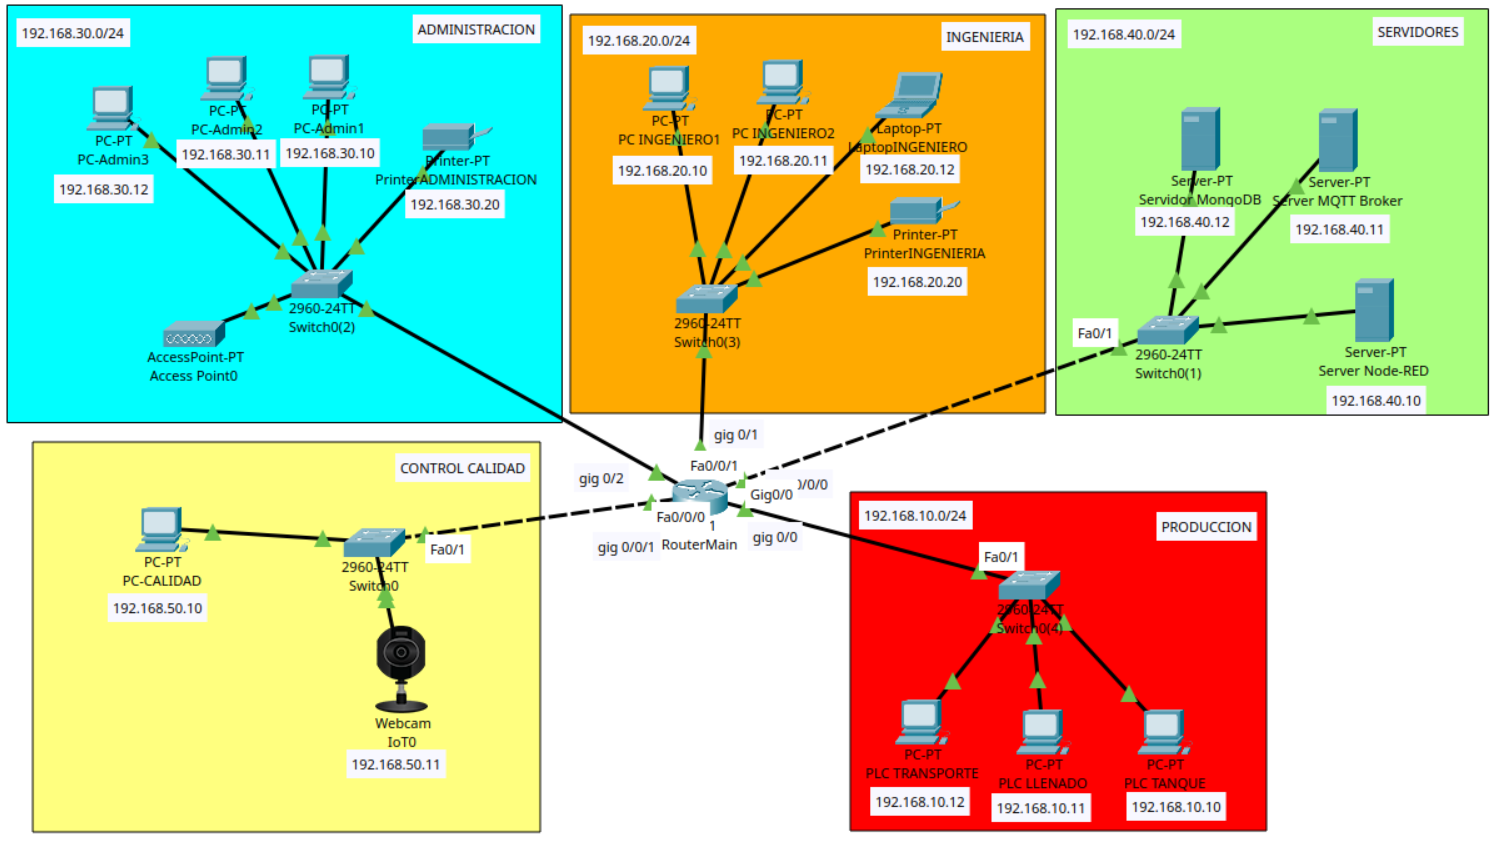
\includegraphics[width=0.85\textwidth]{assets/cap7/7.8.png}
\caption{Topologia de red corporativa en Cisco Packet Tracer}
\label{fig:topologia-packet-tracer}
\end{figure}

\subsection{Componentes de interconexion}

El nucleo de la red es un router Cisco 2911 con las siguientes funciones:

\begin{itemize}
    \item Tres interfaces GigabitEthernet (Gig0/0, Gig0/1, Gig0/2) conectan directamente las redes de produccion, ingenieria y administracion.
    \item Un modulo HWIC-4ESW anade cuatro puertos FastEthernet que, mediante SVIs (Switch Virtual Interfaces), dan servicio a las redes de servidores (VLAN 40) y calidad (VLAN 50) a traves de switches externos.
    \item El router actua como gateway de todas las subredes y encamina el trafico entre ellas.
\end{itemize}

\begin{figure}[H]
\centering
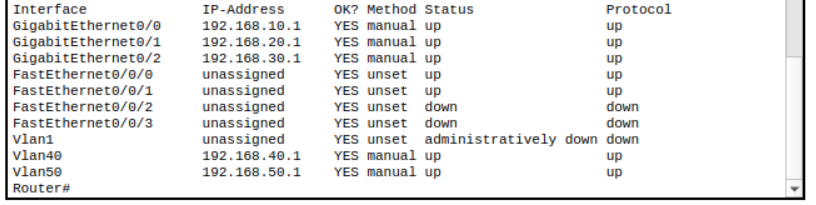
\includegraphics[width=0.8\textwidth]{assets/cap7/7.9.png}
\caption{Configuracion del router con interfaces y SVIs}
\label{fig:router-config}
\end{figure}

\subsection{Esquema de direccionamiento}

\begin{table}[H]
\centering
\small
\caption{Direccionamiento IP de la red corporativa}
\label{tab:direccionamiento-red}
\begin{tabularx}{\textwidth}{@{}lccc@{}}
\toprule
\textbf{Red} & \textbf{Rango} & \textbf{Gateway} & \textbf{Dispositivos} \\
\midrule
Produccion (OT) & 192.168.10.0/24 & 192.168.10.1 & 3 PLCs \\
Ingenieria & 192.168.20.0/24 & 192.168.20.1 & 2 PCs \\
Administracion & 192.168.30.0/24 & 192.168.30.1 & 3 PCs \\
Servidores (DMZ) & 192.168.40.0/24 & 192.168.40.1 & MQTT, Node-RED, MongoDB \\
Control calidad & 192.168.50.0/24 & 192.168.50.1 & PC + camara IP \\
WiFi corporativo & 192.168.100.0/24 & 192.168.100.1 & AP + dispositivos moviles \\
\bottomrule
\end{tabularx}
\end{table}

A continuacion se detalla la funcion de cada departamento dentro de la arquitectura de la planta:

\begin{itemize}
    \item \textbf{Produccion (OT)}: es el nucleo operativo de la planta. Los tres PLCs controlan respectivamente el nivel del tanque de agua, el sistema de llenado de botellas y el transporte de las mismas a traves de las cintas. Esta red debe estar aislada del trafico IT para evitar que incidencias ofimaticas afecten a la produccion. Solo los servidores de la DMZ tienen acceso controlado a ella para la recogida de datos via MQTT.
    \item \textbf{Ingenieria}: destinada al personal tecnico encargado de la supervision, el mantenimiento y la optimizacion de la linea de produccion. Dispone de herramientas de monitorizacion y acceso al dashboard de Node-RED para visualizar el estado en tiempo real de los PLCs y sensores. Tambien es el punto desde el que se realizan actualizaciones de firmware y ajustes de parametros.
    \item \textbf{Administracion}: area de gestion de la planta donde se manejan los indicadores de produccion, la facturacion y la logistica. El personal administrativo accede a los datos historicos del sistema a traves del dashboard, pero no tiene capacidad de escribir comandos sobre los dispositivos OT.
    \item \textbf{Servidores (DMZ)}: zona intermedia que actua como puente entre OT e IT. Alberga el broker MQTT que recibe los datos de produccion, el servidor Node-RED que los procesa y los visualiza, y la base de datos MongoDB que los persiste. Ningun dispositivo externo accede directamente a los PLCs; todo el flujo pasa por esta capa intermedia, lo que anade seguridad y desacopla los sistemas.
    \item \textbf{Control de calidad}: estacion de inspeccion visual donde un operario revisa el producto terminado mediante una camara IP. Los resultados de la inspeccion pueden realimentar el sistema para ajustar parametros de produccion.
    \item \textbf{WiFi corporativo}: proporciona conectividad inalambrica para dispositivos moviles del personal (tabletas, portatiles) dentro de las instalaciones, permitiendo la supervision desde cualquier punto de la planta sin necesidad de estar conectado fisicamente a la red cableada.
\end{itemize}

\subsection{Funcionamiento y flujo de datos}

El flujo de informacion replica el diseno de la memoria tecnica:

\begin{enumerate}
    \item Los PLCs de la red de produccion (OT) adquieren datos de sensores y estados de actuadores.
    \item Estos datos se publican via MQTT hacia el servidor Broker en la red de servidores (192.168.40.10).
    \item Node-RED (192.168.40.11) se suscribe al Broker, procesa los mensajes JSON y los visualiza en el dashboard.
    \item Los datos historicos se persisten en MongoDB (192.168.40.12).
    \item El personal de ingenieria (192.168.20.x) y administracion (192.168.30.x) accede al dashboard a traves del router.
\end{enumerate}

\subsection{Flujo de datos entre departamentos}

El flujo de informacion replica el diseno de la memoria tecnica, cruzando los distintos departamentos de la planta:

\begin{enumerate}
    \item Los PLCs de la red de produccion (OT) adquieren datos de sensores y estados de actuadores en tiempo real.
    \item Estos datos se publican via MQTT hacia el servidor Broker en la red de servidores (192.168.40.10), en la DMZ.
    \item Node-RED (192.168.40.11) se suscribe al Broker, procesa los mensajes JSON y los visualiza en el dashboard.
    \item Los datos historicos se persisten en MongoDB (192.168.40.12) para su consulta posterior.
    \item El personal de ingenieria (192.168.20.x) accede al dashboard para monitorizar y ajustar la produccion.
    \item El personal de administracion (192.168.30.x) consulta los indicadores historicos y las metricas de rendimiento.
    \item El operario de control de calidad (192.168.50.x) registra las inspecciones y puede activar alarmas si detecta anomalias.
\end{enumerate}

\begin{figure}[H]
\centering
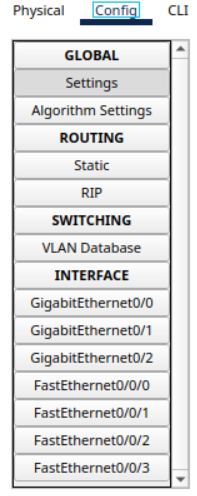
\includegraphics[width=0.27\textwidth]{assets/cap7/7.10.png}
\caption{Tabla de encaminamiento del router}
\label{fig:tabla-rutas}
\end{figure}

El modelo valida que la arquitectura de comunicaciones planteada en la memoria es viable y que la segmentacion en subredes permite aislar el trafico OT del IT, mejorando la seguridad y la gestion de la red industrial.\bigskip


\section{Conclusiones y Recomendaciones Tecnicas}

\begin{enumerate}
    \item \textbf{La arquitectura I2C + MQTT es funcional} y ha sido estabilizada tras las correcciones de anti-spam, manejo de errores y eliminacion de operaciones bloqueantes en ISRs.
    \item \textbf{Las versiones de simulacion permiten validar la logica} sin depender del hardware de campo.
    \item \textbf{El sistema implementa una arquitectura de tres capas completa} (adquisicion, orquestacion/visualizacion, persistencia).
    \item \textbf{Recomendaciones para produccion:}
    \begin{itemize}
        \item Implementar autenticacion TLS en MQTT.
        \item Anadir watchdog software en los esclavos.
        \item Considerar un buffer circular o heartbeat entre Master y Esclavos.
        \item Documentar el esquema electrico completo (pines, alimentacion, pull-ups I2C, adaptacion 3.3V/5V).
    \end{itemize}
\end{enumerate}


\section{Coste de la Instalacion}

El sistema descrito en este capitulo simula un entorno de produccion que, de implementarse en una planta industrial real, requeriria una inversion en equipamiento, sensores, actuadores e infraestructura de comunicacion. A continuacion se desglosan los costes estimados, asumiendo que la planta ya dispone de elementos estructurales como tanques de agua, depositos y obra civil.

\subsection{Componentes considerados}

\begin{itemize}
    \item \textbf{Cintas transportadoras}: se requieren 3 unidades para el transporte de botellas entre etapas, con motorreductores y variadores de velocidad. Coste estimado: 6.000\,\texteuro{} cada una.
    \item \textbf{PLC industrial}: se sustituyen los ESP32 por PLCs compactos (tipo Siemens S7-1200 o similar) para garantizar robustez y estandar industrial. Se necesitan 3 unidades. Coste estimado: 1.200\,\texteuro{} cada uno.
    \item \textbf{Sensores de presencia}: 6 sensores inductivos o fotoelectricos distribuidos en las estaciones. Coste estimado: 150\,\texteuro{} cada uno.
    \item \textbf{Sensor de nivel de agua}: sensor ultrasonico o de presion para el tanque. Coste estimado: 400\,\texteuro{}.
    \item \textbf{Sensorica adicional}: finales de carrera, sensores de posicion y paros de emergencia (10 unidades). Coste estimado: 120\,\texteuro{} cada uno.
    \item \textbf{Actuadores}: electrovalvulas para el sistema de llenado (2 unidades, 350\,\texteuro{} cada una) y bombas industriales (1 unidad, 900\,\texteuro{}).
    \item \textbf{Cableado y canalizaciones}: mangueras apantalladas para senales, cable de potencia para motores y canaletas. Coste estimado: 2.000\,\texteuro{}.
    \item \textbf{Cuadro electrico y armario de control}: incluye fuentes de alimentacion, protectores magnetotermicos, contactores y reles. Coste estimado: 3.500\,\texteuro{}.
    \item \textbf{Infraestructura de red}: switch industrial Ethernet, cableado estructurado y punto de acceso WiFi industrial. Coste estimado: 1.500\,\texteuro{}.
    \item \textbf{Panel HMI}: pantalla tactil para operacion local (7 pulgadas). Coste estimado: 1.800\,\texteuro{}.
    \item \textbf{Puesto de supervision}: ordenador industrial con Node-RED y MongoDB. Coste estimado: 2.500\,\texteuro{}.
    \item \textbf{Integracion y puesta en marcha}: ingenieria de diseno, programacion de PLCs, configuracion de red y pruebas. Coste estimado: 8.000\,\texteuro{}.
\end{itemize}

\subsection{Resumen de costes}

\begin{table}[H]
\centering
\small
\caption{Presupuesto estimado de la instalacion}
\label{tab:presupuesto}
\begin{tabularx}{\textwidth}{@{}lXr@{}}
\toprule
\textbf{Concepto} & \textbf{Descripcion} & \textbf{Importe} \\
\midrule
Cintas transportadoras & 3 uds. & 18.000\,\texteuro{} \\
PLC industriales & 3 uds. (S7-1200 o similar) & 3.600\,\texteuro{} \\
Sensores de presencia & 6 uds. inductivos/fotoelectricos & 900\,\texteuro{} \\
Sensor de nivel & 1 ud. ultrasonico/presion & 400\,\texteuro{} \\
Sensorica adicional & 10 uds. finales de carrera + emergencia & 1.200\,\texteuro{} \\
Electrovalvulas & 2 uds. & 700\,\texteuro{} \\
Bomba industrial & 1 ud. & 900\,\texteuro{} \\
Cableado y canalizaciones & Mangueras, canaletas, conectores & 2.000\,\texteuro{} \\
Cuadro electrico & Armario, protecciones, contactores & 3.500\,\texteuro{} \\
Infraestructura de red & Switch industrial, cableado, WiFi & 1.500\,\texteuro{} \\
Panel HMI & Pantalla tactil 7'' & 1.800\,\texteuro{} \\
Puesto de supervision & PC industrial + software & 2.500\,\texteuro{} \\
Integracion y puesta en marcha & Ingenieria, programacion, pruebas & 8.000\,\texteuro{} \\
\midrule
\textbf{Total estimado} & & \textbf{45.000\,\texteuro{}} \\
\bottomrule
\end{tabularx}
\end{table}

\subsection{Costes de mantenimiento}

Una vez en operacion, la instalacion requiere un mantenimiento anual estimado en los siguientes conceptos:

\begin{itemize}
    \item \textbf{Mantenimiento preventivo}: revision trimestral de sensores, actuadores y cableado. Coste estimado: 1.200\,\texteuro{}/ano.
    \item \textbf{Mantenimiento correctivo}: sustitucion de componentes por desgaste (sensores, reles, contactos). Coste estimado: 800\,\texteuro{}/ano.
    \item \textbf{Actualizacion de software}: parches de seguridad, actualizaciones de Node-RED y MongoDB. Coste estimado: 600\,\texteuro{}/ano.
    \item \textbf{Soporte tecnico}: contrato de asistencia remota y visitas programadas. Coste estimado: 1.500\,\texteuro{}/ano.
\end{itemize}

\textbf{Coste de mantenimiento anual total estimado: 4.100\,\texteuro{}}.


\section{Planificacion}

Para llevar a cabo la implementacion del sistema en una planta industrial real, se propone una planificacion en cinco fases distribuidas en un plazo total estimado de 16 semanas.

\subsection{Fases del proyecto}

\begin{enumerate}
    \item \textbf{Fase de diseno y definicion (semanas 1--3)}:
    \begin{itemize}
        \item Analisis de requisitos funcionales y tecnicos.
        \item Definicion de la arquitectura del sistema y seleccion de componentes.
        \item Diseno del esquema electrico y de comunicaciones.
        \item Elaboracion del presupuesto detallado.
    \end{itemize}
    \item \textbf{Fase de adquisicion e infraestructura (semanas 4--6)}:
    \begin{itemize}
        \item Compra de materiales, sensores, actuadores y PLCs.
        \item Instalacion del cuadro electrico, cableado y canalizaciones.
        \item Montaje de la infraestructura de red (switch, acceso WiFi).
    \end{itemize}
    \item \textbf{Fase de desarrollo e integracion (semanas 7--11)}:
    \begin{itemize}
        \item Programacion de los PLCs (logica de control y maquina de estados).
        \item Configuracion del protocolo I2C entre los nodos.
        \item Implementacion del broker MQTT y los topics de comunicacion.
        \item Desarrollo del dashboard en Node-RED y conexion con MongoDB.
        \item Pruebas unitarias de cada subsistema por separado.
    \end{itemize}
    \item \textbf{Fase de pruebas y puesta en marcha (semanas 12--14)}:
    \begin{itemize}
        \item Integracion de todos los subsistemas y pruebas de conjunto.
        \item Verificacion de la maquina de estados y los flujos de datos.
        \item Pruebas de estres y tolerancia a fallos en la comunicacion I2C y MQTT.
        \item Formacion del personal operario en el manejo del HMI y el dashboard.
    \end{itemize}
    \item \textbf{Fase de operacion supervisada y cierre (semanas 15--16)}:
    \begin{itemize}
        \item Operacion supervisada con acompanamiento tecnico.
        \item Ajustes finos de parametros y temporizaciones.
        \item Entrega de documentacion tecnica y manuales de operacion.
        \item Cierre del proyecto y revision de resultados.
    \end{itemize}
\end{enumerate}

\subsection{Diagrama temporal resumido}

\begin{table}[H]
\centering
\small
\caption{Cronograma del proyecto}
\label{tab:cronograma}
\begin{tabularx}{\textwidth}{@{}lXXXXX@{}}
\toprule
\textbf{Fase} & \textbf{Sem. 1--3} & \textbf{Sem. 4--6} & \textbf{Sem. 7--11} & \textbf{Sem. 12--14} & \textbf{Sem. 15--16} \\
\midrule
Diseno y definicion & $\bullet$ & & & & \\
Adquisicion e infraestructura & & $\bullet$ & & & \\
Desarrollo e integracion & & & $\bullet$ & & \\
Pruebas y puesta en marcha & & & & $\bullet$ & \\
Operacion supervisada y cierre & & & & & $\bullet$ \\
\bottomrule
\end{tabularx}
\end{table}



